% ----- Consignes exo 1 ----- %
\begin{td-exo}[Flots --- 3pts]\,\\ % 1
    Calculer un flot maximal sur le réseau de transport ci-dessous, commençant par une augmentation de flot le long du chemin \(sadbep\).
    En expliquant comment l'obtenir, donner une coupe minimale du réseau.

    \ffigbox[\FBwidth]{%
\caption{\centering Réseau de transport initial}\label{Fig:exam_blanc_ex_1_1}
}{
    \fbox{
        \begin{tikzpicture}[scale=1, main node/.style={circle, draw, fill=blue!20, inner sep=1pt, font=\scriptsize, minimum size=6mm}]
            % les sommets initiaux
            \node[main node] (s) at (-3,0) {\(s\)};
            \node[main node] (p) at (3,0) {\(p\)};

            \node[main node] (a) at (-1,2) {\(a\)};
            \node[main node] (b) at (-1,0) {\(b\)};
            \node[main node] (c) at (-1,-2) {\(c\)};

            \node[main node] (d) at (1,2) {\(d\)};
            \node[main node] (e) at (1,0) {\(e\)};
            \node[main node] (f) at (1,-2) {\(f\)};

            % les arcs avec capacités
            \draw[-{Stealth}] (s) -- node[above left] {\(4\)} (a);
            \draw[-{Stealth}] (s) -- node[above] {\(5\)} (b);
            \draw[-{Stealth}] (s) -- node[below left] {\(4\)} (c);

            \draw[-{Stealth}] (a) -- node[above] {\(5\)} (d);

            \draw[-{Stealth}] (b) -- node[above] {\(6\)} (e);
            \draw[-{Stealth}] (b) -- node[left] {\(9\)} (f);

            \draw[-{Stealth}] (c) -- node[below] {\(1\)} (f);

            \draw[-{Stealth}] (d) -- node[above right] {\(2\)} (b);
            \draw[-{Stealth}] (d) -- node[above right] {\(3\)} (p);

            \draw[-{Stealth}] (e) -- node[right] {\(9\)} (c);
            \draw[-{Stealth}] (e) -- node[below right] {\(9\)} (p);

            \draw[-{Stealth}] (f) -- node[below right] {\(1\)} (p);
        \end{tikzpicture}
    }
}
\end{td-exo}

% ----- Solutions exo 1 ----- %
\iftoggle{showsolutions}{
	\begin{td-sol}[]\,\\ % 1
		Commençons par retirer \(sadbep\) au réseau pour obtenir le réseau résiduel suivant:

        \input{../assets/tikz/exam_blanc_ex_1_2.tex}

        Ensuite, on peut faire passer 2 de flot par \(sbdp\) et 1 de flot par \(scfp\) pour obtenir les graphes suivants:

		\begin{figure}[H]
	\CenterFloatBoxes{}		% centers the floatrow contents horizontally
	\begin{floatrow}
		\input{../assets/tikz/exam_blanc_ex_2_2_a.tex}

		\input{../assets/tikz/exam_blanc_ex_2_2_b.tex}
	\end{floatrow}
\end{figure}

        Ensuite, on peut faire passer 1 de flot par \(sadp\) et 3 par \(sbep\):

        \input{../assets/tikz/exam_blanc_ex_1_4.tex}

        Il ne reste plus qu'à faire passer une dernière fois 1 de flot par \(sadbep\) et on aura fini:

        \begin{figure}[H]
	\CenterFloatBoxes{}		% centers the floatrow contents horizontally
	\begin{floatrow}
		\ffigbox[\FBwidth]{%
\caption{\centering Réseau de transport initial après la dernière étape}\label{Fig:exam_blanc_ex_1_5_a}
}{
    \fbox{
        \begin{tikzpicture}[scale=1, main node/.style={circle, draw, fill=blue!20, inner sep=1pt, font=\scriptsize, minimum size=6mm}]
            % les sommets initiaux
            \node[main node] (s) at (-3,0) {\(s\)};
            \node[main node] (p) at (3,0) {\(p\)};

            \node[main node] (a) at (-1,2) {\(a\)};
            \node[main node] (b) at (-1,0) {\(b\)};
            \node[main node] (c) at (-1,-2) {\(c\)};

            \node[main node] (d) at (1,2) {\(d\)};
            \node[main node] (e) at (1,0) {\(e\)};
            \node[main node] (f) at (1,-2) {\(f\)};

            % les arcs avec capacités
            \draw[-{Stealth}, draw=red] (s) to node[above left] {\(4/4\)} (a);
            \draw[-{Stealth}, draw=blue] (s) to node[above] {\(5/5\)} (b);
            \draw[-{Stealth}, draw=blue] (s) to node[below left] {\(1/4\)} (c);

            \draw[-{Stealth}, draw=red] (a) to node[above] {\(4/5\)} (d);

            \draw[-{Stealth}, draw=red] (b) to node[above] {\(6/6\)} (e);
            \draw[-{Stealth}] (b) to node[left] {\(9\)} (f);

            \draw[-{Stealth}, draw=blue] (c) to node[below] {\(1/1\)} (f);

            \draw[-{Stealth}, draw=red] (d) to node[right] {\(1/2\)} (b);
            \draw[-{Stealth}, draw=blue] (d) to node[above right] {\(3/3\)} (p);

            \draw[-{Stealth}] (e) to node[right] {\(9\)} (c);
            \draw[-{Stealth}, draw=red] (e) to node[above] {\(6/9\)} (p);
            \draw[-{Stealth}, draw=blue] (f) to node[below right] {\(1/1\)} (p);
        \end{tikzpicture}
    }
}

		\ffigbox[\FBwidth]{%
\caption{\centering Réseau résiduel après avoir retiré un dernier flot de 1 par \(sadbep\)}\label{Fig:exam_blanc_ex_1_5_b}
}{
    \fbox{
        \begin{tikzpicture}[scale=1, main node/.style={circle, draw, fill=blue!20, inner sep=1pt, font=\scriptsize, minimum size=6mm}]
            % les sommets initiaux
            \node[main node] (s) at (-3,0) {\(s\)};
            \node[main node] (p) at (3,0) {\(p\)};

            \node[main node] (a) at (-1,2) {\(a\)};
            \node[main node] (b) at (-1,0) {\(b\)};
            \node[main node] (c) at (-1,-2) {\(c\)};

            \node[main node] (d) at (1,2) {\(d\)};
            \node[main node] (e) at (1,0) {\(e\)};
            \node[main node] (f) at (1,-2) {\(f\)};

            % les arcs avec capacités
            \draw[-{Stealth}, draw=blue] (s) to node[below left] {\(3\)} (c);

            \draw[-{Stealth}, draw=red, bend left] (a) to node[above] {\(1\)} (d);
            \draw[-{Stealth}, draw=red, bend left] (d) to node[above] {\(4\)} (a);

            \draw[-{Stealth}, draw=red] (e) to node[above] {\(6\)} (b);
            \draw[-{Stealth}] (b) to node[left] {\(9\)} (f);

            \draw[-{Stealth}, draw=blue] (f) to node[below] {\(1\)} (c);

            \draw[-{Stealth}, draw=red, bend left] (d) to node[right] {\(1/2\)} (b);
            \draw[-{Stealth}, draw=red] (b) to node[left] {\(1/2\)} (d);

            \draw[-{Stealth}] (e) to node[right] {\(9\)} (c);
            \draw[-{Stealth}, draw=red] (e) to node[above] {\(3\)} (p);

            \node[inner sep=12pt, fit=(s) (c), name=SCFIT] {};

            \draw[green!60, thick, fill=green!20, opacity=0.4, rotate around={45:(SCFIT.center)}]
                (SCFIT.center) ellipse [x radius=0.9cm, y radius=2cm];


        \end{tikzpicture}
    }
}
	\end{floatrow}
\end{figure}

        On a trouvé un flot maximal de valeur 10.
        Une coupe minimale est donnée par l'ensemble des sommets atteignables depuis \(s\) dans le réseau résiduel final, soit \(\{s, c\}\).

	\end{td-sol}
}{}


% ----- Consignes exo 2 ----- %
\begin{td-exo}[Indépendant dans les subcubiques --- 5pts]\,\\ % 2
    Un graphe \(G = (V,E)\) est dit \defemph{subcubique} si tous ses sommets ont degré au plus 3, c'est à dire si \(\forall v\in V, \mathsf{deg}_G(v) \leq 3\).
    Le but de l'exercice est de donner des bornes sur \(\alpha(G)\), la taille du plus grand ensemble indépendant (ou stable) de \(G\) en fonction de \(n\), le nombre de sommets de \(G\).
    \begin{enumerate}
        \item On commence par fournir une borne inférieure pour \(\alpha(G)\).
        \begin{enumerate}
            \item Montrer que si \(x\) est un sommet de \(G\) et \(I\) un indépendant de \(G \setminus \left( x\cup N_G(x) \right)\) alors \(I \cup \{x\}\) est un indépendant de \(G\).
            \item En déduire, par récurrence sur \(n\), que tout graphe subcubique à \(n\) sommets admet un indépendant de taille au moins \(\lceil \frac{n}{4} \rceil\).
        \end{enumerate}

        \item On suppose maintenant que \(G\) est cubique (c'est à dire \(\forall v\in V, \mathsf{deg}_G(v) = 3\)) et on va établir une borne supérieure pour \(\alpha(G)\).
        \begin{enumerate}
            \item Soit \(X\) un indépendant de \(G\). En fonction de la taille de \(X\), calculer le nombre d'arêtes, noté \(e(X, \ol{X})\), entre \(X\) et son complémentaire.
            \item En déduire que \(|X| \leq |\ol{X}|\) puis que \(|X| \leq \lfloor \frac{n}{2} \rfloor\).
        \end{enumerate}

        \item Donner deux exemples de graphes cubiques \(G_1\) et \(G_2\) sur \(n\) sommets tels que \(\alpha(G_1) = \frac{n}{4}\) et \(\alpha(G_2) = \frac{n}{2}\). Si possible, vous donnerez des exemples pour \(n\) arbitrairement grand.
    \end{enumerate}
\end{td-exo}

% ----- Solutions exo 2 ----- %
\iftoggle{showsolutions}{
	\begin{td-sol}[]\, % 2
		\begin{enumerate}
            \item On fournit une borne inférieure pour \(\alpha(G)\).
            \begin{enumerate}
                \item\label{exb:ex2:q1} Soit \(x\) un sommet de \(G\) et \(I\) un indépendant de \(G \setminus \left( x\cup N_G(x) \right)\).
                Soit \(y\) un sommet de \(I\). 
                
                Si \(y\) est un voisin de \(x\) alors \(y \in N_G(x)\) ce qui contredit le fait que \(y\) est dans \(G \setminus \left( x\cup N_G(x) \right)\).
                Donc \(y\) n'est pas un voisin de \(x\). 
                
                Alors, tout sommet de \(I\) n'est pas voisin de \(x\) donc \(I \cup \{x\}\) est un indépendant de \(G\).

                \item On montre par récurrence (forte) sur \(n\) que tout graphe subcubique à \(n\) sommets admet un indépendant de taille au moins \(\lceil \frac{n}{4} \rceil\).
                
                Pour \(n=1\), le graphe subcubique est réduit à un sommet isolé qui est bien un indépendant de taille \(1 \geq \lceil \frac{1}{4} \rceil\).
                
                Supposons que la propriété est vraie pour tout graphe subcubique à \(k\) sommets (avec \(1 \leq k < n\)) et montrons-la pour un graphe subcubique \(G\) à \(n\) sommets.
                
                Soit \(G\) un graphe subcubique à \(n\) sommets.
                Soit \(x\) un sommet de \(G\).
                
                Le graphe \(G' = G \setminus \left( x\cup N_G(x) \right)\) est subcubique (car \(G\) l'est) et possède au moins \(n-4\) sommets (ceux de départ, moins \(x\) et au plus ses 3 voisins).
                Par hypothèse de récurrence, il admet un indépendant \(I\) de taille au moins \(\lceil \frac{n-4}{4} \rceil\).
                
                D'après~\eqref{exb:ex2:q1}, \(I \cup \{x\}\) est un indépendant de \(G\) de taille au moins \(\lceil \frac{n-4}{4} \rceil + 1\).
            \end{enumerate}
            Donc \(G\) admet un indépendant de taille au moins \(\lceil \frac{n}{4} \rceil\).

            \item On suppose maintenant que \(G\) est cubique et on établit une borne supérieure pour \(\alpha(G)\).
            \begin{enumerate}
                \item Soit \(X\) un indépendant de \(G\).
                Chaque sommet de \(X\) possède 3 arêtes qui le relient à des sommets de \(\ol{X}\) (car \(G\) est cubique et \(X\) est un indépendant).
                Donc \(e(X, \ol{X}) = 3|X|\).

                \item Au mieux, tout triplet de sommets de \(X\) est relié à un même triplet de sommets de \(\ol{X}\).
                Donc \(|X| \leq |\ol{X}|\).

                De plus, on a \(X \sqcup \ol{X} = V\) donc \(|X| + |\ol{X}| = n\). Comme \(|X| \leq |\ol{X}|\), on a forcément \(|X| \leq \lfloor \frac{n}{2} \rfloor\).
            \end{enumerate}

            \item On peut utiliser les graphes suivants:
            \begin{itemize}
                \item Pour \(G_1\), on peut prendre une collection de copies du graphe suivant (le nombre de copies dépend de \(n\)):
                
                \ffigbox[\FBwidth]{%
\caption{\centering Graphe cubique utilisé pour construire \(G_1\)}\label{Fig:exam_blanc_ex_2_1}
}{
    \fbox{
        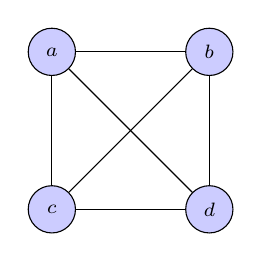
\begin{tikzpicture}[scale=1, main node/.style={circle, draw, fill=blue!20, inner sep=1pt, font=\scriptsize, minimum size=6mm}]
            % graphe complet de taille 4
            \node[main node] (a) at (0,2) {\(a\)};
            \node[main node] (b) at (2,2) {\(b\)};
            \node[main node] (c) at (0,0) {\(c\)};
            \node[main node] (d) at (2,0) {\(d\)};
            
            \draw (a) -- (b);
            \draw (a) -- (c);
            \draw (a) -- (d);

            \draw (b) -- (c);
            \draw (b) -- (d);

            \draw (c) -- (d);

        \end{tikzpicture}
    }
}

                Chaque copie possède un indépendant de taille 1 (par exemple le sommet central) et le graphe est cubique.
                Donc pour \(n\) suffisamment grand, on peut obtenir un graphe cubique à \(n\) sommets avec un indépendant de taille \(\frac{n}{4}\).

                \item Pour \(G_2\), on peut prendre une collection de copies du graphe suivant (le nombre de copies dépend de \(n\)):
                
                \vspace{0.2cm}
                \ffigbox[\FBwidth]{%
\caption{\centering Graphe cubique utilisé pour construire \(G_2\)}\label{Fig:exam_blanc_ex_2_2}
}{
    \fbox{
        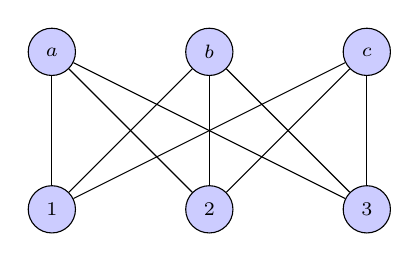
\begin{tikzpicture}[scale=1, main node/.style={circle, draw, fill=blue!20, inner sep=1pt, font=\scriptsize, minimum size=6mm}]
            % graphe biparti 3 3 de taille 6
            \node[main node] (a) at (0,2) {\(a\)};
            \node[main node] (b) at (2,2) {\(b\)};
            \node[main node] (c) at (4, 2) {\(c\)};

            \node[main node] (1) at (0,0) {\(1\)};
            \node[main node] (2) at (2,0) {\(2\)};
            \node[main node] (3) at (4,0) {\(3\)};
            
            % on relie chaque sommet en haut à tous ceux en bas
            \draw (a) -- (1);
            \draw (a) -- (2);
            \draw (a) -- (3);

            \draw (b) -- (1);
            \draw (b) -- (2);
            \draw (b) -- (3);

            \draw (c) -- (1);
            \draw (c) -- (2);
            \draw (c) -- (3);

        \end{tikzpicture}
    }
}

                Chaque copie possède un indépendant de taille 3 (par exemple les trois sommets en haut) et le graphe est cubique.
                Donc pour \(n\) suffisamment grand, on peut obtenir un graphe cubique à \(n\) sommets avec un indépendant de taille \(\frac{n}{2}\).
            \end{itemize}
        \end{enumerate}
	\end{td-sol}
}{}


% ----- Consignes exo 3 ----- %
\begin{td-exo}[Couplage max --- 3pts]\,\\ % 3
    Dans le graphe suivant, appliquer l'algorithme d'Edmonds pour calculer un couplage maximum, en sachant que le couplage \(\left\{ be, ci, hp \right\}\) a déjà été précalculé. Au cours de votre déroulement d'algorithme, vous devrez, à au moins une reprise, contracter un blossom.

    \vspace{0.2cm}
    \ffigbox[\FBwidth]{%
\caption{\centering Graphe avec couplage \(\{be, ci, hp\}\) précalculé}\label{Fig:exam_blanc_ex_3_1}
}{
    \fbox{
        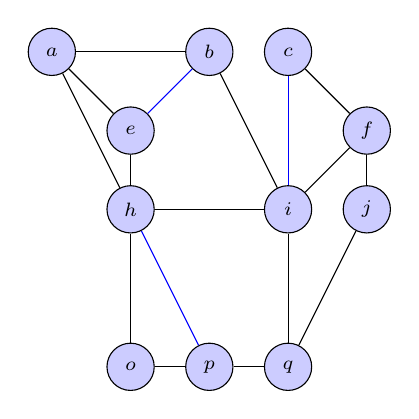
\begin{tikzpicture}[scale=1, main node/.style={circle, draw, fill=blue!20, inner sep=1pt, font=\scriptsize, minimum size=6mm}]
            % les sommets initiaux
            \node[main node] (a) at (-2,2) {\(a\)};
            \node[main node] (b) at (0,2) {\(b\)};
            \node[main node] (c) at (1,2) {\(c\)};

            \node[main node] (e) at (-1,1) {\(e\)};
            \node[main node] (f) at (2,1) {\(f\)};

            \node[main node] (h) at (-1,0) {\(h\)};
            \node[main node] (i) at (1,0) {\(i\)};
            \node[main node] (j) at (2, 0) {\(j\)};

            \node[main node] (o) at (-1, -2) {\(o\)};
            \node[main node] (p) at (0, -2) {\(p\)};
            \node[main node] (q) at (1, -2) {\(q\)};

            % les aretes
            \draw[] (a) -- (b);
            \draw[] (a) -- (e);
            \draw[] (a) -- (h);

            \draw[draw=blue] (b) -- (e);
            \draw[] (b) -- (i);

            \draw[] (c) -- (f);
            \draw[draw=blue] (c) -- (i);
            \draw[] (e) -- (h);

            \draw[] (f) -- (i);
            \draw[] (f) -- (j);

            \draw[] (h) -- (i);
            \draw[] (h) -- (o);
            \draw[draw=blue] (h) -- (p);

            \draw[] (i) -- (q);

            \draw[] (j) -- (q);

            \draw[] (o) -- (p);

            \draw[] (p) -- (q);
        \end{tikzpicture}
    }
}
\end{td-exo}

% ----- Solutions exo 3 ----- %
\iftoggle{showsolutions}{
	\begin{td-sol}[]\,\\ % 3   
        On commence par rajouter le couplage initial:

        \vspace{0.2cm}
        \input{../assets/tikz/exam_blanc_ex_3_2.tex}

        Contractons maintenant des blossoms. On peut commencer par le blossom \(cfi\):

        \vspace{0.2cm}
        \ffigbox[\FBwidth]{%
\caption{\centering Graphe après contraction du blossom \(cfi\)}\label{Fig:exam_blanc_ex_3_3}
}{
    \fbox{
        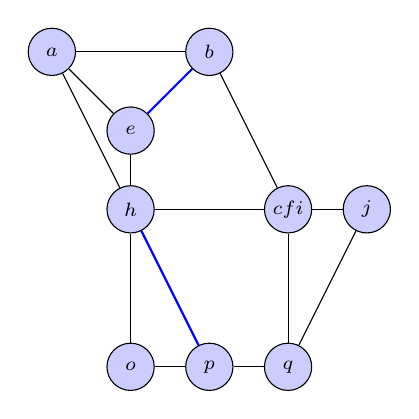
\begin{tikzpicture}[scale=1, main node/.style={circle, draw, fill=blue!20, inner sep=1pt, font=\scriptsize, minimum size=6mm}]
            % les sommets initiaux
            \node[main node] (a) at (-2,2) {\(a\)};
            \node[main node] (b) at (0,2) {\(b\)};
            % \node[main node] (c) at (1,2) {\(c\)};

            \node[main node] (e) at (-1,1) {\(e\)};
            % \node[main node] (f) at (2,1) {\(f\)};

            \node[main node] (h) at (-1,0) {\(h\)};
            \node[main node] (cfi) at (1,0) {\(cfi\)};
            \node[main node] (j) at (2, 0) {\(j\)};

            \node[main node] (o) at (-1, -2) {\(o\)};
            \node[main node] (p) at (0, -2) {\(p\)};
            \node[main node] (q) at (1, -2) {\(q\)};

            % les aretes
            \draw[] (a) -- (b);
            \draw[] (a) -- (e);
            \draw[] (a) -- (h);

            \draw[draw=blue, thick] (b) -- (e);
            \draw[] (b) -- (cfi);

            % \draw[] (c) -- (f);
            % \draw[draw=blue, thick] (c) -- (i);
            \draw[] (e) -- (h);

            % \draw[] (f) -- (i);
            \draw[] (cfi) -- (j);

            \draw[] (h) -- (cfi);
            \draw[] (h) -- (o);
            \draw[draw=blue, thick] (h) -- (p);

            \draw[] (cfi) -- (q);

            \draw[] (j) -- (q);

            \draw[] (o) -- (p);

            \draw[] (p) -- (q);
        \end{tikzpicture}
    }
}

        Ensuite on peut contracter le blossom \(cfijq\):

        \vspace{0.2cm}
        \input{../assets/tikz/exam_blanc_ex_3_4.tex}

        Cherchons maintenant des chemins augmentants. 
        On part d'un sommet non saturé, ici \(a\), et on trouve le chemin augmentant \(ae-eb-bcfijq\).
        On augment alors le couplage:

        \vspace{0.2cm}
        \input{../assets/tikz/exam_blanc_ex_3_5.tex}

        Il ne reste qu'un seul sommet non saturé \(o\) donc on a fini de trouver des chemins augmentants.
        Il faut maintenant décontracter nos blossoms pour retrouver le couplage maximum:

        \vspace{0.2cm}
        \ffigbox[\FBwidth]{%
\caption{\centering Graphe après décontraction du blossom \(cfijq\)}\label{Fig:exam_blanc_ex_3_6}
}{
    \fbox{
        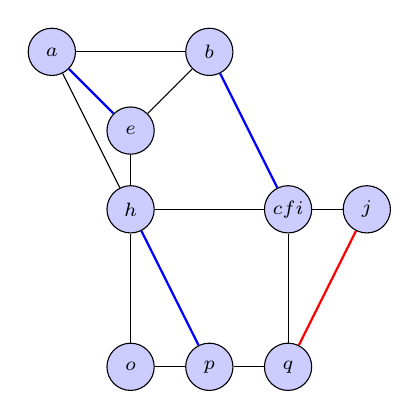
\begin{tikzpicture}[scale=1, main node/.style={circle, draw, fill=blue!20, inner sep=1pt, font=\scriptsize, minimum size=6mm}]
            % les sommets initiaux
            \node[main node] (a) at (-2,2) {\(a\)};
            \node[main node] (b) at (0,2) {\(b\)};
            % \node[main node] (c) at (1,2) {\(c\)};

            \node[main node] (e) at (-1,1) {\(e\)};
            % \node[main node] (f) at (2,1) {\(f\)};

            \node[main node] (h) at (-1,0) {\(h\)};
            \node[main node] (cfi) at (1,0) {\(cfi\)};
            \node[main node] (j) at (2, 0) {\(j\)};

            \node[main node] (o) at (-1, -2) {\(o\)};
            \node[main node] (p) at (0, -2) {\(p\)};
            \node[main node] (q) at (1, -2) {\(q\)};

            % les aretes
            \draw[] (a) -- (b);
            \draw[draw=blue, thick] (a) -- (e);
            \draw[] (a) -- (h);

            \draw[] (b) -- (e);
            \draw[draw=blue, thick] (b) -- (cfi);

            % \draw[] (c) -- (f);
            % \draw[draw=blue, thick] (c) -- (i);
            \draw[] (e) -- (h);

            % \draw[] (f) -- (i);
            \draw[] (cfi) -- (j);

            \draw[] (h) -- (cfi);
            \draw[] (h) -- (o);
            \draw[draw=blue, thick] (h) -- (p);

            \draw[] (cfi) -- (q);

            \draw[draw=red, thick] (j) -- (q);

            \draw[] (o) -- (p);

            \draw[] (p) -- (q);
        \end{tikzpicture}
    }
}

        Enfin, on décontracte le blossom \(cfi\) pour obtenir le couplage maximum final:
        
        \vspace{0.2cm}
        \input{../assets/tikz/exam_blanc_ex_3_7.tex}

        On voit alors notre couplage maximum de taille 5:
        \begin{equation*}
            \left\{
                ae, bi, cf, hp, qj
            \right\}.
        \end{equation*}
	\end{td-sol}
}{}


% ----- Consignes exo 4 ----- %
\begin{td-exo}[Miam! --- 5pts]\,\\ % 4
    Trois étudiants affamés, nommés \(E_1, E_2\) et \(E_3\), se retrouvent pour manger 6 pizzas, notées \(P_1, \ldots, P_6\).
    Chaque étudiant veut manger 2 pizzas exactement. Les étudiants ont les contraintes alimentaires suivantes:
    \begin{itemize}
        \item \(E_1\) qui déteste les champignons, ne veut manger que les pizzas \(P_1, P_4\) et \(P_5\).
        \item \(E_2\) qui est allergique au chorizo, ne veut manger que les pizzas \(P_2, P_5\) et \(P_6\).
        \item \(E_3\) qui ne digère pas les anchois, ne veut manger que les pizzas \(P_1, P_2, P_3\) et \(P_6\).
    \end{itemize}
    On souhaite savoir si il est possible de répartir les 6 pizzas afin de satisfaire les choix des étudiants.
    \begin{enumerate}
        \item Construire le graphe biparti \(H_{(E, P)}\) défini sur \(\left\{P_1, \ldots, P_6\right\} \cup \left\{E_1, E_2, E_3\right\}\) et dont les arêtes sont \(\{P_i E_j : \) si \(E_j\) veut manger la pizza \(P_i\}\).
        \item Quelle structure souhaite-t-on trouver dans \(H_{(E, P)}\) pour garantir une solution au problème?
        \item Une \defemph{copie} d'un sommet \(x\) dans un graphe \(G\) est un sommet \(y\) non-adjacent à \(x\) et dont le voisinage est identique à celui de \(x\). A partir du graphe \(H_{(E, P)}\), on construit le graphe \(H_{(E, P)}'\) en ajoutant une copie pour chaque sommet \(E_i\). Sans preuve, quelle structure souhaite-t-on trouver dans \(H_{(E, P)}'\) pour garantir que les trois étudiants peuvent se répartir les six pizzas en respectant leurs choix?
        \item Résoudre le problème (en utilisant un algorithme du cours \(\ldots\)).
        \item Plus généralement, soit \(k\geq 2\) fixé, le \defemph{centre} d'un graphe biparti complet \(K_{1, k}\) est le sommet de ce graphe qui n'est pas une feuille. 
        Etant donné un graphe biparti \(G = ((A, B), E)\), on souhaite déterminer si \(G\) peut être (sommet-)~partitionné en graphes \(K_{1, k}\) dont les centres sont tous dans \(A\). 
        Donner un algorithme de résolution en temps polynomial pour ce problème. Prouver la validité de votre algorithme.
    \end{enumerate}
\end{td-exo}

% ----- Solutions exo 4 ----- %
\iftoggle{showsolutions}{
	\begin{td-sol}[]\, % 4
		\begin{enumerate}
            \item Le graphe biparti \(H_{(E, P)}\) est le suivant:

            \vspace{0.2cm}
            \ffigbox[\FBwidth]{%
\caption{\centering Graphe biparti \(H_{(E, P)}\) avec les préférences culinaires des étudiants}\label{Fig:exam_blanc_ex_4_1}
}{
    \fbox{
        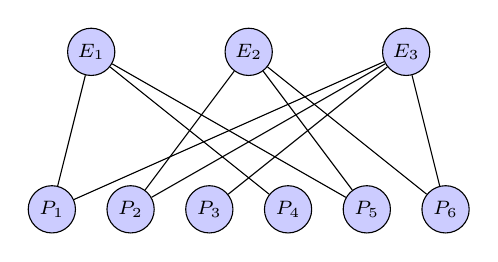
\begin{tikzpicture}[scale=1, main node/.style={circle, draw, fill=blue!20, inner sep=1pt, font=\scriptsize, minimum size=6mm}]
            % les sommets initiaux
            \node[main node] (E1) at (-2,2) {\(E_1\)};
            \node[main node] (E2) at (0,2) {\(E_2\)};
            \node[main node] (E3) at (2,2) {\(E_3\)};
            
            \node[main node] (P1) at (-2.5,0) {\(P_1\)};
            \node[main node] (P2) at (-1.5,0) {\(P_2\)};
            \node[main node] (P3) at (-0.5,0) {\(P_3\)};
            \node[main node] (P4) at (0.5,0) {\(P_4\)};
            \node[main node] (P5) at (1.5,0) {\(P_5\)};
            \node[main node] (P6) at (2.5,0) {\(P_6\)};

            % les aretes
            \draw[] (E1) -- (P1);
            \draw[] (E1) -- (P4);
            \draw[] (E1) -- (P5);

            \draw[] (E2) -- (P2);
            \draw[] (E2) -- (P5);
            \draw[] (E2) -- (P6);

            \draw[] (E3) -- (P1);
            \draw[] (E3) -- (P2);
            \draw[] (E3) -- (P3);
            \draw[] (E3) -- (P6);
        \end{tikzpicture}
    }
}

            \item On souhaite trouver deux couplages disjoints saturant les sommets \(E_1, E_2\) et \(E_3\).

            \item On souhaite trouver un couplage parfait dans le graphe \(H_{(E, P)}'\) suivant:

            \vspace{0.2cm}
            \input{../assets/tikz/exam_blanc_ex_4_2.tex}

            \item On utilise l'algorithme d'Edmonds pour trouver un couplage maximum dans \(H_{(E, P)}'\).
            On commence par trouver un chemin augmentant à partir de \(E_1\):

            \vspace{0.2cm}
            \ffigbox[\FBwidth]{%
\caption{\centering Graphe biparti \(H_{(E, P)}'\) après calcul du couplage \(E_1 P_1\)}\label{Fig:exam_blanc_ex_4_3}
}{
    \fbox{
        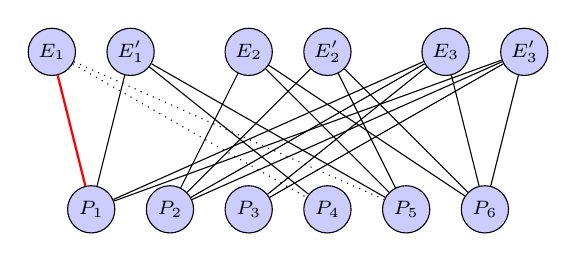
\begin{tikzpicture}[scale=1, main node/.style={circle, draw, fill=blue!20, inner sep=1pt, font=\scriptsize, minimum size=6mm}]
            % les sommets initiaux
            \node[main node] (E1) at (-3,2) {\(E_1\)};
            \node[main node] (E1p) at (-2,2) {\(E_1'\)};
            \node[main node] (E2) at (-0.5,2) {\(E_2\)};
            \node[main node] (E2p) at (0.5,2) {\(E_2'\)};
            \node[main node] (E3) at (2,2) {\(E_3\)};
            \node[main node] (E3p) at (3,2) {\(E_3'\)};
            
            \node[main node] (P1) at (-2.5,0) {\(P_1\)};
            \node[main node] (P2) at (-1.5,0) {\(P_2\)};
            \node[main node] (P3) at (-0.5,0) {\(P_3\)};
            \node[main node] (P4) at (0.5,0) {\(P_4\)};
            \node[main node] (P5) at (1.5,0) {\(P_5\)};
            \node[main node] (P6) at (2.5,0) {\(P_6\)};

            % les aretes
            \draw[draw=red, thick] (E1) -- (P1);
            \draw[dotted] (E1) -- (P4);
            \draw[dotted] (E1) -- (P5);

            \draw[] (E1p) -- (P1);
            \draw[] (E1p) -- (P4);
            \draw[] (E1p) -- (P5);

            \draw[] (E2) -- (P2);
            \draw[] (E2) -- (P5);
            \draw[] (E2) -- (P6);

            \draw[] (E2p) -- (P2);
            \draw[] (E2p) -- (P5);
            \draw[] (E2p) -- (P6);

            \draw[] (E3) -- (P1);
            \draw[] (E3) -- (P2);
            \draw[] (E3) -- (P3);
            \draw[] (E3) -- (P6);

            \draw[] (E3p) -- (P1);
            \draw[] (E3p) -- (P2);
            \draw[] (E3p) -- (P3);
            \draw[] (E3p) -- (P6);
        \end{tikzpicture}
    }
}
            
            Dans la suite on omettra les arêtes à partir de sommets étudiants déjà dans le couplage.

            Puis on trouve un chemin augmentant à partir de \(E_1'\):

            \vspace{0.2cm}
            \input{../assets/tikz/exam_blanc_ex_4_4.tex}

            Ensuite pour \(E_2\):

            \vspace{0.2cm}
            \input{../assets/tikz/exam_blanc_ex_4_5.tex}

            Et pour \(E_2'\):

            \vspace{0.2cm}
            \input{../assets/tikz/exam_blanc_ex_4_6.tex}

            Enfin pour \(E_3\):

            \vspace{0.2cm}
            \input{../assets/tikz/exam_blanc_ex_4_7.tex}

            Et pour \(E_3'\):

            \vspace{0.2cm}
            \ffigbox[\FBwidth]{%
\caption{\centering Graphe biparti \(H_{(E, P)}'\) après rajout de \(E_3' P_6\) dans le couplage}\label{Fig:exam_blanc_ex_4_8}
}{
    \fbox{
        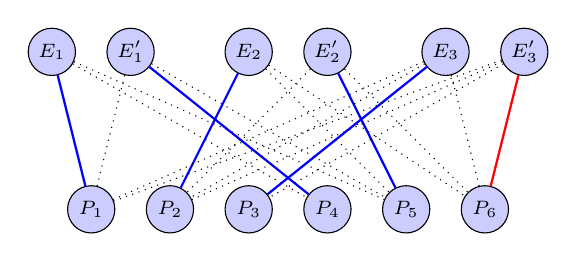
\begin{tikzpicture}[scale=1, main node/.style={circle, draw, fill=blue!20, inner sep=1pt, font=\scriptsize, minimum size=6mm}]
            % les sommets initiaux
            \node[main node] (E1) at (-3,2) {\(E_1\)};
            \node[main node] (E1p) at (-2,2) {\(E_1'\)};
            \node[main node] (E2) at (-0.5,2) {\(E_2\)};
            \node[main node] (E2p) at (0.5,2) {\(E_2'\)};
            \node[main node] (E3) at (2,2) {\(E_3\)};
            \node[main node] (E3p) at (3,2) {\(E_3'\)};
            
            \node[main node] (P1) at (-2.5,0) {\(P_1\)};
            \node[main node] (P2) at (-1.5,0) {\(P_2\)};
            \node[main node] (P3) at (-0.5,0) {\(P_3\)};
            \node[main node] (P4) at (0.5,0) {\(P_4\)};
            \node[main node] (P5) at (1.5,0) {\(P_5\)};
            \node[main node] (P6) at (2.5,0) {\(P_6\)};

            % les aretes
            \draw[draw=blue, thick] (E1) -- (P1);
            \draw[dotted] (E1) -- (P4);
            \draw[dotted] (E1) -- (P5);

            \draw[dotted] (E1p) -- (P1);
            \draw[draw=blue, thick] (E1p) -- (P4);
            \draw[dotted] (E1p) -- (P5);

            \draw[draw=blue, thick] (E2) -- (P2);
            \draw[dotted] (E2) -- (P5);
            \draw[dotted] (E2) -- (P6);

            \draw[dotted] (E2p) -- (P2);
            \draw[draw=blue, thick] (E2p) -- (P5);
            \draw[dotted] (E2p) -- (P6);

            \draw[dotted] (E3) -- (P1);
            \draw[dotted] (E3) -- (P2);
            \draw[draw=blue, thick] (E3) -- (P3);
            \draw[dotted] (E3) -- (P6);

            \draw[dotted] (E3p) -- (P1);
            \draw[dotted] (E3p) -- (P2);
            \draw[dotted] (E3p) -- (P3);
            \draw[draw=red, thick] (E3p) -- (P6);
        \end{tikzpicture}
    }
}

            On a trouvé un couplage parfait dans \(H_{(E, P)}'\) donc les trois étudiants peuvent se répartir les six pizzas comme suit:
            \begin{equation*}
                \begin{cases}
                    E_1 \text{ mange } P_1 \text{ et } P_4\\
                    E_2 \text{ mange } P_2 \text{ et } P_5\\
                    E_3 \text{ mange } P_3 \text{ et } P_6
                \end{cases}
            \end{equation*}

            \item Pas encore rédigé.
        \end{enumerate}
	\end{td-sol}
}{}


% ----- Consignes exo 5 ----- %
\begin{td-exo}[Graphes auto-complémentaires --- 4pts]\,\\ % 5
    Un graphe \(G\) est dit \defemph{auto-complémentaire} si \(G\) est isomorphe à son complémentaire \(\ol{G}\).
    \begin{enumerate}
        \item Justifier que \(P_4\) et \(C_5\) sont auto-complémentaires.
        \item Montrer que tout graphe auto-complémentaire est connexe.
        \item En notant \(n\) le nombre de sommets de \(G\), calculer le nombre d'arêtes d'un graphe auto-complémentaire en fonction de \(n\).
        \item En déduire que \(n \equiv 0 \text{ ou } 1 \mod 4\).
        \item\label{exb:q5:1} Soit \(G\) un graphe auto-complémentaire et \(P\) un chemin de longueur 3 (c'est à dire avec 4 sommets).
        On note \(G'\) le graphe obtenu depuis \(G \cup P\) en reliant le premier et le dernier sommet de \(P\) à tous les sommets de \(G\).
        Montrer que \(G'\) est auto-complémentaire.
        \item En déduire que pour tout \(n\) avec \(n \equiv 0 \text{ ou } 1 \mod 4\), il existe un graphe auto-complémentaire à \(n\) sommets.
    \end{enumerate}
\end{td-exo}

% ----- Solutions exo 5 ----- %
\iftoggle{showsolutions}{
	\begin{td-sol}[]\, % 5
		\begin{enumerate}
            \item Dessinons ces graphes et leurs complémentaires pour comprendre visuellement ce qui se passe:

            \vspace{0.2cm}
            \begin{figure}[H]
	\CenterFloatBoxes{}		% centers the floatrow contents horizontally
	\begin{floatrow}
		\input{../assets/tikz/exam_blanc_ex_5_1_a.tikz}

		\ffigbox[\FBwidth]{%
\caption{\centering Graphe \(C_5\) de départ}\label{Fig:exam_blanc_ex_5_1_b}
}{
    \fbox{
        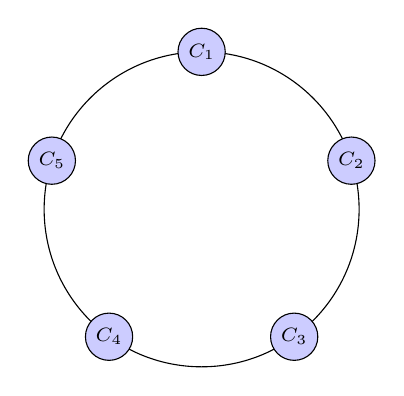
\begin{tikzpicture}[scale=1, main node/.style={circle, draw, fill=blue!20, inner sep=1pt, font=\scriptsize, minimum size=6mm}]
            % le cercle de départ 
            \draw (0, 0) circle [radius=2];
            
            % les sommets initiaux
            \node[main node] (1) at (90:2)  {\(C_1\)};
            \node[main node] (2) at (18:2)  {\(C_2\)};
            \node[main node] (3) at (-54:2) {\(C_3\)};
            \node[main node] (4) at (-126:2){\(C_4\)};
            \node[main node] (5) at (-198:2){\(C_5\)};
            
        \end{tikzpicture}
    }
}
	\end{floatrow}
\end{figure}

            Lorsqu'on prend leur complémentaire, on obtient les graphes suivants:

            \vspace{0.2cm}
            \begin{figure}[H]
	\CenterFloatBoxes{}		% centers the floatrow contents horizontally
	\begin{floatrow}
		\ffigbox[\FBwidth]{%
\caption{\centering Complémentaire du graphe \(P_4\)}\label{Fig:exam_blanc_ex_5_1_a}
}{
    \fbox{
        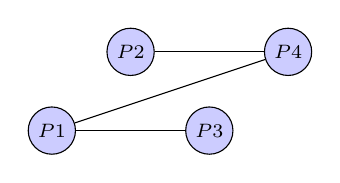
\begin{tikzpicture}[scale=1, main node/.style={circle, draw, fill=blue!20, inner sep=1pt, font=\scriptsize, minimum size=6mm}]
            % les sommets initiaux
            \node[main node] (P1) at (0,0) {\(P1\)};
            \node[main node] (P2) at (1,1) {\(P2\)};
            \node[main node] (P3) at (2,0) {\(P3\)};
            \node[main node] (P4) at (3,1) {\(P4\)};

            % les aretes
            \draw[] (P1) -- (P3);
            \draw[] (P1) -- (P4);

            \draw[] (P2) -- (P4);
        \end{tikzpicture}
    }
}


		\ffigbox[\FBwidth]{%
\caption{\centering Complémentaire du graphe \(C_5\)}\label{Fig:exam_blanc_ex_5_2_b}
}{
    \fbox{
        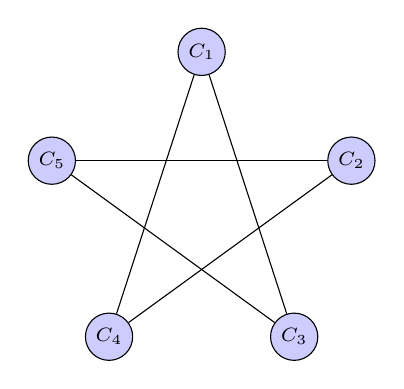
\begin{tikzpicture}[scale=1, main node/.style={circle, draw, fill=blue!20, inner sep=1pt, font=\scriptsize, minimum size=6mm}]
            % les sommets initiaux
            \node[main node] (C1) at (90:2)  {\(C_1\)};
            \node[main node] (C2) at (18:2)  {\(C_2\)};
            \node[main node] (C3) at (-54:2) {\(C_3\)};
            \node[main node] (C4) at (-126:2){\(C_4\)};
            \node[main node] (C5) at (-198:2){\(C_5\)};

            % les aretes
            \draw[] (C1) -- (C3);
            \draw[] (C1) -- (C4);
            
            \draw[] (C2) -- (C4);
            \draw[] (C2) -- (C5);
            
            \draw[] (C3) -- (C5);
        \end{tikzpicture}
    }
}
	\end{floatrow}
\end{figure}

            On voit alors clairement qu'on peut identifier dans ces graphes un unique chemin (respectivement cycle) qui passe par toutes les arêtes et tous les sommets.

            Formellement, on peut définir les fonctions suivantes:
            \begin{equation*}
                f_{P_4} : 
                \begin{cases}
                    P_1 \mapsto P_2\\
                    P_2 \mapsto P_4\\
                    P_3 \mapsto P_1\\
                    P_4 \mapsto P_3
                \end{cases}
                \quad
                f_{C_5} : 
                \begin{cases}
                    C_1 \mapsto C_1\\
                    C_2 \mapsto C_3\\
                    C_3 \mapsto C_5\\
                    C_4 \mapsto C_2\\
                    C_5 \mapsto C_4
                \end{cases}
            \end{equation*}
            qui sont des isomorphismes entre \(P_4\) et \(\ol{P_4}\) (respectivement \(C_5\) et \(\ol{C_5}\)).

            Alors, ces graphes sont bien auto-complémentaires.

            \item Soit \(G\) un graphe non connexe.
            Alors, il existe une partition de \(V(G)\) en deux ensembles non vides \(A\) et \(B\) tels qu'il n'existe pas d'arête entre un sommet de \(A\) et un sommet de \(B\).
            Dans le complémentaire \(\ol{G}\), tous les sommets de \(A\) sont reliés à tous les sommets de \(B\).
            Donc \(\ol{G}\) est connexe.
            Ainsi, \(G\) et \(\ol{G}\) ne peuvent pas être isomorphes (et donc auto-complémentaires).

            Donc tout graphe auto-complémentaire est connexe.

            \item Soit \(G\) un graphe auto-complémentaire à \(n\) sommets.
            On note \(m\) le nombre d'arêtes de \(G\).
            On remarque que le nombre total d'arêtes possibles dans un graphe à \(n\) sommets est \(\frac{n(n-1)}{2}\).
            Comme \(G\) est isomorphe à \(\ol{G}\), on a forcément 
            \begin{equation*}
                \begin{aligned}
                    m = \frac{n(n-1)}{2} - m
                    &\iff 2m = \frac{n(n-1)}{2}\\
                    &\iff m = \frac{n(n-1)}{4}.
                \end{aligned}
            \end{equation*}

            \item Comme \(m\) est un entier, \(\frac{n(n-1)}{4}\) doit être un entier et donc 
            on a forcément \(n(n-1) \equiv 0 \mod 4\), c'est à dire \(n \equiv 0 \text{ ou } 1 \mod 4\).

            \item On se donne un graphe auto-complémentaire \(G\) à \(n\) sommets et un chemin \(P\) de longueur 3.
            On note \(G'\) le graphe obtenu depuis \(G \cup P\) avec le procédé décrit dans l'énoncé~\eqref{exb:q5:1}.
            On a:

            % TODO: replace by the correct figure
            % \vspace{0.2cm}
            % \ffigbox[\FBwidth]{%
\caption{\centering Graphe \(G \cup P\)}\label{Fig:exam_blanc_ex_5_3}
}{
    \fbox{
        \begin{tikzpicture}[scale=1, main node/.style={circle, draw, fill=blue!20, inner sep=1pt, font=\scriptsize, minimum size=6mm}]
            % les sommets de G
            \node[main node] (g1) at (-1, 2) {\(g1\)};
            \node[] (dots) at (-1, 0) {\(\vdots\)};
            \node[main node] (gn) at (-1, -2) {\(g_n\)};

            % les sommets de P
            \node[main node] (p1) at (4, 3) {\(p1\)};
            \node[main node] (p2) at (5, 1) {\(p2\)};
            \node[main node] (p3) at (3, -1) {\(p3\)};
            \node[main node] (p4) at (4, -3) {\(p4\)};

            % on entoure G
            \node[inner sep=12pt, fit=(g1) (gn), name=GFIT] {};

            \draw[green!60, thick, fill=green!20, opacity=0.4]
                (GFIT.center) ellipse [x radius=1.3cm, y radius=2.5cm];
            \node at (GFIT.south) [yshift=-10pt] {\(G\)};

            % les aretes
            % dans P
            \draw (p1) -- (p2);
            \draw (p2) -- (p3);
            \draw (p3) -- (p4);
            
            % entre G et P
            \draw (p1) -- (g1);
            \draw[dashed] (p1) -- (dots);
            \draw (p1) -- (gn);

            \draw (p4) -- (g1);
            \draw[dashed] (p4) -- (dots);
            \draw (p4) -- (gn);
        \end{tikzpicture}
    }
}

            Observons ce qui se passe quand on passe au complémentaire \(\ol{G'}\):

            % TODO: replace by the correct figure
            % \vspace{0.2cm}
            % \ffigbox[\FBwidth]{%
\caption{\centering Complémentaire du graphe \(G \cup P\)}\label{Fig:exam_blanc_ex_5_4}
}{
    \fbox{
        \begin{tikzpicture}[scale=1, main node/.style={circle, draw, fill=blue!20, inner sep=1pt, font=\scriptsize, minimum size=6mm}]
            % les sommets de G
            \node[main node] (g1) at (-1, 2) {\(g1\)};
            \node[] (dots) at (-1, 0) {\(\vdots\)};
            \node[main node] (gn) at (-1, -2) {\(g_n\)};

            % les sommets de P
            \node[main node] (p1) at (4, 3) {\(p1\)};
            \node[main node] (p2) at (5, 1) {\(p2\)};
            \node[main node] (p3) at (3, -1) {\(p3\)};
            \node[main node] (p4) at (4, -3) {\(p4\)};

            % on entoure G
            \node[inner sep=12pt, fit=(g1) (gn), name=GFIT] {};

            \draw[green!60, thick, fill=green!20, opacity=0.4]
                (GFIT.center) ellipse [x radius=1.3cm, y radius=2.5cm];
            \node at (GFIT.south) [yshift=-10pt] {\(G\)};

            % les aretes
            % dans P
            \draw (p1) -- (p3);
            \draw (p1) -- (p4);
            \draw (p2) -- (p4);
            
            % entre G et P
            \draw (p2) -- (g1);
            \draw[dashed] (p2) -- (dots);
            \draw (p2) -- (gn);

            \draw (p3) -- (g1);
            \draw[dashed] (p3) -- (dots);
            \draw (p3) -- (gn);
        \end{tikzpicture}
    }
}

            

            \item Si \(n = 4\) ou \(n = 5\), on peut prendre \(G = P_4\) ou \(G = C_5\).
            Sinon, on peut construire \(G'\) à partir de \(G\) en répétant le procédé 
            décrit en~\eqref{exb:q5:1} pour obtenir un graphe de taille \(n\) (car l'opération 
            ajoute 4 sommets à chaque fois et conserve la propriété d'auto-complémentarité).
        \end{enumerate}
	\end{td-sol}
}{}
